\documentclass[12pt, a4paper]{article}
\usepackage[lmargin =0.5 in, 
rmargin=0.5in, 
tmargin=1in,
bmargin=0.5in]{geometry}
\geometry{letterpaper}
\usepackage{tikz-cd}
\usepackage{amsmath}
\usepackage{amssymb}
\usepackage{blindtext}
\usepackage{titlesec}
\usepackage{enumitem}
\usepackage{fancyhdr}
\usepackage{amsthm}
\usepackage{graphicx}
\usepackage{cool}
\usepackage{thmtools}
\usepackage{hyperref}
\graphicspath{ }					%path to an image

%-------- sexy font ------------%
%\usepackage{libertine}
%\usepackage{libertinust1math}

%\usepackage{mlmodern}				% very nice and classic
%\usepackage[utopia]{mathdesign}
%\usepackage[T1]{fontenc}


\usepackage{mlmodern}
\usepackage{eulervm}
%\usepackage{tgtermes} 				%times new roman
%-------- sexy font ------------%


% Problem Styles
%====================================================================%


\newtheorem{problem}{Problem}


\theoremstyle{definition}
\newtheorem{thm}{Theorem}
\newtheorem{lemma}{Lemma}
\newtheorem{prop}{Proposition}
\newtheorem{cor}{Corollary}
\newtheorem{fact}{Fact}
\newtheorem{defn}{Definition}
\newtheorem{example}{Example}
\newtheorem{question}{Question}

\newtheorem{manualprobleminner}{Problem}

\newenvironment{manualproblem}[1]{%
	\renewcommand\themanualprobleminner{#1}%
	\manualprobleminner
}{\endmanualprobleminner}

\newcommand{\penum}{ \begin{enumerate}[label=\bf(\alph*), leftmargin=0pt]}
	\newcommand{\epenum}{ \end{enumerate} }

% Math fonts shortcuts
%====================================================================%

\newcommand{\ring}{\mathcal{R}}
\newcommand{\N}{\mathbb{N}}                           % Natural numbers
\newcommand{\Z}{\mathbb{Z}}                           % Integers
\newcommand{\R}{\mathbb{R}}                           % Real numbers
\newcommand{\C}{\mathbb{C}}                           % Complex numbers
\newcommand{\F}{\mathbb{F}}                           % Arbitrary field
\newcommand{\Q}{\mathbb{Q}}                           % Arbitrary field
\newcommand{\PP}{\mathcal{P}}                         % Partition
\newcommand{\M}{\mathcal{M}}                         % Mathcal M
\newcommand{\eL}{\mathcal{L}}                         % Mathcal L
\newcommand{\T}{\mathbb{T}}                         % Mathcal T
\newcommand{\U}{\mathcal{U}}                         % Mathcal U\\
\newcommand{\V}{\mathcal{V}}                         % Mathcal V

% symbol shortcuts
%====================================================================%

\newcommand{\bd}{\partial}
\newcommand{\grad}{\nabla}
\newcommand{\lam}{\lambda}
\newcommand{\imp}{\implies}
\newcommand{\all}{\forall}
\newcommand{\exs}{\exists}
\newcommand{\delt}{\delta}
\newcommand{\ep}{\varepsilon}
\newcommand{\ra}{\rightarrow}
\newcommand{\vph}{\varphi}

\newcommand{\ol}{\overline}
\newcommand{\f}{\frac}
\newcommand{\lf}{\lfrac}
\newcommand{\df}{\dfrac}

% bracketting shortcuts
%====================================================================%
\newcommand{\abs}[1]{\left| #1 \right|}
\newcommand{\babs}[1]{\Big|#1\Big|}
\newcommand{\bound}{\Big|}
\newcommand{\BB}[1]{\left(#1\right)}
\newcommand{\dd}{\mathrm{d}}
\newcommand{\artanh}{\mathrm{artanh}}
\newcommand{\Med}{\mathrm{Med}}
\newcommand{\Cov}{\mathrm{Cov}}
\newcommand{\Corr}{\mathrm{Corr}}
\newcommand{\tr}{\mathrm{tr}}
\newcommand{\Range}[1]{\mathrm{range}(#1)}
\newcommand{\Null}[1]{\mathrm{null}(#1)}
\newcommand{\lan}{\langle}
\newcommand{\ran}{\rangle}
\newcommand{\norm}[1]{\left\lVert#1\right\rVert}
\newcommand{\inn}[1]{\lan#1\ran}
\newcommand{\op}[1]{\operatorname{#1}}
\newcommand{\bmat}[1]{\begin{bmatrix}#1\end{bmatrix}}
\newcommand{\pmat}[1]{\begin{pmatrix}#1\end{pmatrix}}
\newcommand{\vmat}[1]{\begin{vmatrix}#1\end{vmatrix}}

\newcommand{\amogus}{{\bigcap}\kern-0.8em\raisebox{0.3ex}{$\subset$}}
\newcommand{\Note}{\textbf{Note: }}
\newcommand{\Aside}{{\bf Aside: }}
%restriction
%\newcommand{\op}[1]{\operatorname{#1}}
%\newcommand{\done}{$$\mathcal{QED}$$}

%====================================================================%


\setlength{\parindent}{0pt}      	% No paragraph indentations
\pagestyle{fancy}
\fancyhf{}							% fancy header

\setcounter{secnumdepth}{0}			% sections are numbered but numbers do not appear
\setcounter{tocdepth}{2} 			% no subsubsections in toc

%template
%====================================================================%
%\begin{manualproblem}{1}
%Spivak.
%\end{manualproblem}

%\begin{proof}[Solution]
%\end{proof}

%----------- or -----------%

%\begin{problem} 		
%\end{problem}	

%\penum
%	\item
%\epenum
%====================================================================%


\newcommand{\Course}{351}
\newcommand{\hwNumber}{2}

%preamble

\title{}
\author{A.N.}
\date{\today}
\lhead{\Course A\hwNumber}
\rhead{\thepage}
%\cfoot{\thepage}


%====================================================================%
\begin{document}



\begin{problem}
\end{problem}
\penum
\item By the Cauchy-Riemann equations, we have 
	$$u_{xx} + u_{yy} = (u_x)_x + (u_y)_y =v_{xy} - v_{yx}=0 .$$
	Similarly, for $v$ we have
	$$v_{xx} +v_{yy} = -v_{xy} + v_{xy} = 0. $$
\item Given a harmonic $u(x,y)$ we can define $v(x,y) = \int_0^y u_x(x,t) dy$. 
	We compute that $$v_y = \frac{\partial}{\partial y} \int_0^y u_x(x,t) dt = u_x. $$
	Similarly, we have $$v_x = \int_0^y u_{xx} (x,t) dt = \int_0^y -u_{yy}(x,t) dt = -u_y.$$
	Thus we can find the conjugate harmonic function to $u$. 
\epenum
 \newpage 
\begin{problem}
\end{problem}
\penum
\item We have shown in class that the characteristics of this equation are lines of the form $y=x+c$ for $c\in \R$. 
	$$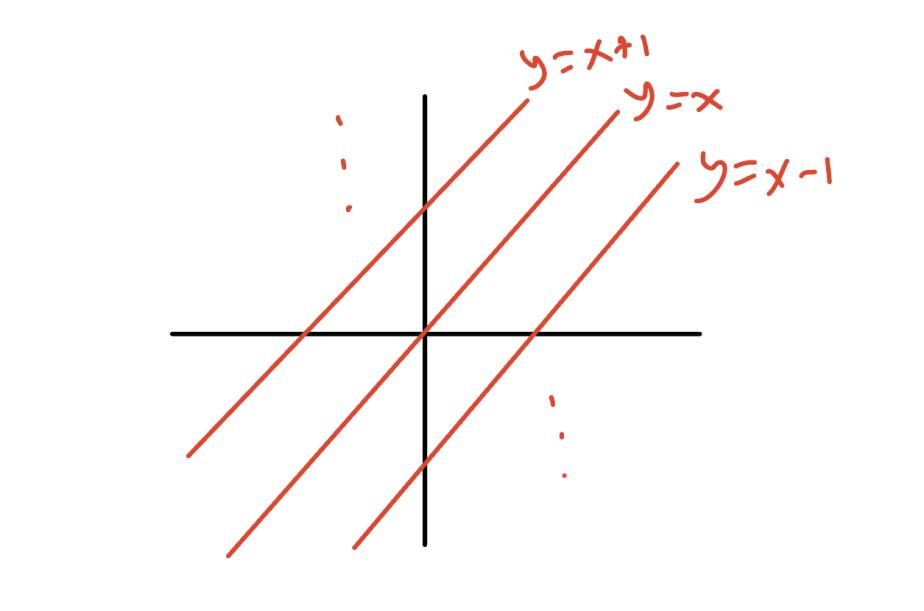
\includegraphics[width=0.5\textwidth]{mat351A2Q2a.jpg}.$$
\item We solve the inhomogenous PDE now, with the boundary value $u(x,0) = f(x)$. We write $u(x(t), y(t))$, and get the following system of ODE's from out PDE through any point $(x_0,0)$:
	$$\begin{cases}
		\dot{x} = 1 & x(0) = x_0\\
		\dot{y} = 1 & y(0) = 0 \\
		\dot{u} = 1 & u(x,0) = f(x)
	\end{cases}$$
Solving this, we get $x(t) = t+x_0, y(t) = t$ and $u(x,y) = t+ f(x_0)$. Since $x_0 = x-y$, and $y=t$ we have that $u(x,y) = y + f(x-y)$
\epenum
 \newpage 
\begin{problem}
\end{problem}
We parametrize the characteristic curves as $(x(t),y(t))$, through the point $(0,y_0)$, and get the system of ODE's from $u(x(t), y(t))$: 
$$\begin{cases}
	\dot{x}(t) = y(t) & x(0) = 0\\
	\dot{y}(t) = x(t) & y(0) = y_0 \\ 
	\dot{z}(s) =0 & z(0) = \cos y_0
\end{cases}$$
We solve for $x(t) ,y(t)$ as $x(t) = Ce^t + De^{-t}, y(t) = Ce^t + De^{-t}$. With initial conditions we get that $x(t) = y_0 \sinh t , y(t) = y_0 \cosh t $. We can rewrite $x,y$ as $y+x = y_0 e^t, y-x=y_0 e^{-t}$. Thus we have that $y_0^2 = y^2 - x^2$. Therefore $u(x,y) = \cos \left(\sqrt{y^2-x^2}  \right)$. 
$$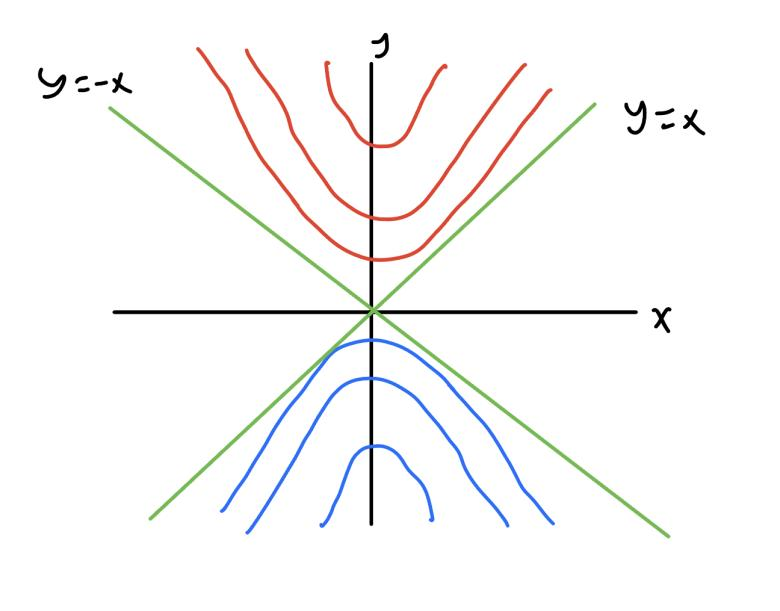
\includegraphics[width = 0.5\textwidth]{mat351A2Q3.jpg}$$
We have unique solutions on the regions above $y=x, y= -x$, and below $y=x, y=-x$. If we expand the region to include the union of the lines $y=x, y=-x$, we will lose uniqueness. If we take the initial value at $(0,0)$, we will have two solutions, namely $y=x,y=-x$ passing through this point. 
 \newpage 
\begin{problem}
\end{problem}
\penum
\item Consider the coordinate change of $\xi = \frac{t+x}{2} , \eta = \frac{t-x}{2}$. Using the chain rule, we compute that $$u_t =\frac{1}{2} u_\xi +  \frac{1}{2} u_\eta $$ and $$u_{tt} =\frac{1}{4} u_{\xi \xi} + \frac{1}{2} u_{\xi \eta} + \frac{1}{4} u_{\eta \eta}. $$
Similarly, we have that $$u_{xx} = \frac{1}{4} u_{\xi \xi } - \frac{1}{2} u_{\eta \xi} + \frac{1}{4} u_{\eta \eta}.$$
Therefore we have that $$0 = u_{tt} - u_{xx} = u_{\eta \xi}.$$
\item For $c\neq 0$, we make the coordinate change $\xi = \frac{t+c x}{2} , \eta = \frac{t-cx}{2}$.	We compute that $$u_{xx} = c^2 \left(\frac{1}{4} u_{\xi \xi } + \frac{1}{2} u_{\xi \eta} + \frac{1}{4} u_{\eta\eta}   \right),$$
	and $u_{tt} $ remains unchanged from $a)$. We have once again that this coordinate change yields $u_{\eta \xi}=0$. 
\item Given that $u_{\eta \xi}=0$ , we have that $u_\eta = f(\eta)$ for some $f$, and similarly. $u_\xi = g(\xi)$ for some $g$. Therefore we have that $$u = G(\xi) + F(\eta) = F\left(\frac{t+x}{2}\right) + G\left(\frac{t-x}{2}\right) = G(t+x) + F(t-x), $$
for arbitrary functions $F,G$. 
Given the boundary values $u(0,x) = f(x), u_t(0,x) = 0$, we have that $$F(x) + G(x)= f(x) , F^\prime (x) -G^\prime(x) = 0. \implies G = F+c.$$
Therefore we can write $2F(x) + c = f(x)$ which implies that $F(x) = \frac{f(x) -c}{2}, G(x) = \frac{f(x)+ c}{2}. $  Thus we have that $$u(x,y) = \frac{f(t+x) + f(t-x)}{2}.$$ 
\item 
	Yes this is unique. Suppose $u,v$ solve the boundary value problem given in $c)$.
Then $u-v$ satisfies the same boundary value problem with $f(x) =0$. The same equations hold, writing $(u-v) = F(t+x) + G(x-t), $ we get that $F^\prime(x) = G^\prime(x)$, and $F(x) + G(x) = 0$. This implies that $F = G+c$ and so $2G + c = 0$. So $G = c$, similarly $F = 2c$. The initial value tells us that $F=G = 0$. Therefore $u=v$. 
\epenum
 \newpage 
\begin{problem}
\end{problem}
By the previous question, we have that the solution $u$ takes the form
$$u(x,y) = F(x+t) + G(x-t). $$
The boundary values give us that $$f(x) = u(x,x) =F(2x) + G(0)\implies F(x+t) = f \left(\frac{x+t}{2}\right) $$
The normal vector to $t=x$ is $(-1,1)$, so we can compute the normal derivative as: 
$$u_\nu = \bmat{F^\prime(x+t) + G^\prime(x-t) & F^\prime(x+t) - G^\prime(x-t)} \cdot \pmat{-1 \\ 1} =0.$$
This is a problem for existence unless $g(x) = 0$. If $g=0$, uniqueness becomes a problem. Since $G$ is constant on the boundary, we can choose an arbitrary $G$ of the form $G(x-t)$, with $G(0)=0$, and add it to our solution $f \left( \frac{x+2}{2} \right)$. Therefore this is not a well posed boundary value problem. 
\end{document}
